\documentclass[presentation.tex]{subfiles}
\begin{document}

\maketitle


\section{Structure for multipatch}
\paragraph{}
We are trying here to answer to the following questions: 
\begin{itemize}
	\item What kind of information do we need to store in each patch? 
	\item What kind of information do the patches need to exchange? 
\end{itemize}


\subsection{Type of global space splitting}
\paragraph{}
The splitting of the global space into patches is currently not fixed. However we can encounter three types of sticking: 
\begin{itemize}
	\item simple interface which sticks two whole edges together; 
	\item T-joint which sticks several edges to one edge of a patch; 
	\item X-point where the sticking is only on one point. 
\end{itemize}

\paragraph{}
Each patch is defined on a logical domain and maps the mesh points to a physical domain (cf. Fig. \ref{log_phy_domain}). 
The figure Fig. \ref{Patches_logical_dom} gives examples of the different stickings on the logical domain. 

\begin{figure}[!h]
\centering
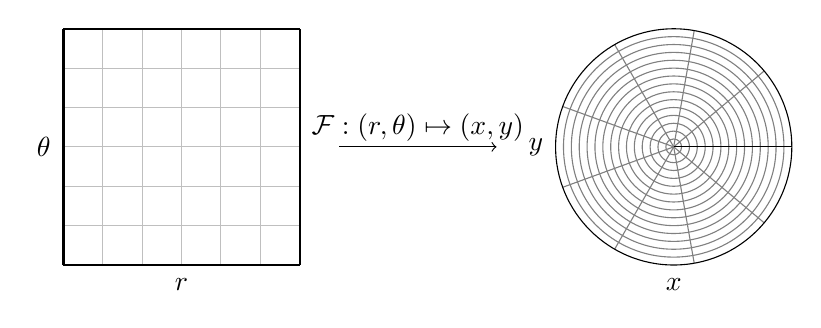
\begin{tikzpicture}[xscale = 1, yscale = 1]
	% logical grid
	\draw[lightgray] (0,0) grid [step = 0.5] (3,3);
	\draw[thick] (0,0) grid [step = 3] (3,3);
	
	\node at (-0.25, 1.5) {$\theta$}; 
	\node at (1.5, -0.25) {$r$}; 
	
	% mapping
	\draw[->] (3.5, 1.5) -- (5.5, 1.5); 
	\node at (4.5,1.75) {$\mathcal{F}:(r,\theta)\mapsto(x,y)$}; 
	
	\begin{scope}[xshift = 7.75cm, yshift = 1.5cm]	
		% physical grid
		\def\Rmax{1.5}
		\foreach \r in {0, 0.1, ...,\Rmax} {
		    \draw[gray] (0,0) circle (\r);
		}
		\foreach \theta in {0, 40,...,360} {
    			\draw[gray] (0,0) -- (\theta:\Rmax);
		}
		
		\draw[black] (0,0) circle (\Rmax);
		\draw[black] (0,0) -- (0:\Rmax);
		
		\node at (-1.75, 0) {$y$}; 
		\node at (0, -1.75) {$x$}; 
	\end{scope}
\end{tikzpicture}
\caption{\label{log_phy_domain} Mapping from the logical domain to the physical domain. Example with a circular mapping.}
\end{figure}

\begin{figure}[!h]
\begin{subfigure}{0.5\textwidth}
\centering
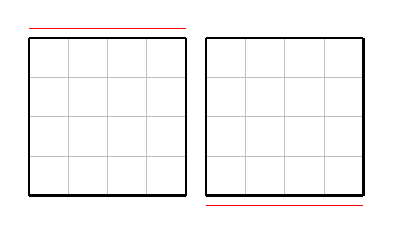
\begin{tikzpicture}[xscale = 1, yscale = 1]
	\draw[lightgray] (0,0) grid [step = 0.5] (2,2);
	\draw[thick] (0,0) grid [step = 2] (2,2);
	
	\draw[red] (0,2.125) -- (2,2.125);
	
	\begin{scope}[shift={(2.25,0)}]
		\draw[lightgray] (0,0) grid [step = 0.5] (2,2);
		\draw[thick] (0,0) grid [step = 2] (2,2);
		
		\draw[red] (0,-0.125) -- (2,-0.125);
	\end{scope}
\end{tikzpicture}
\caption{Simple interface.}
\end{subfigure}
\begin{subfigure}{0.5\textwidth}
\centering
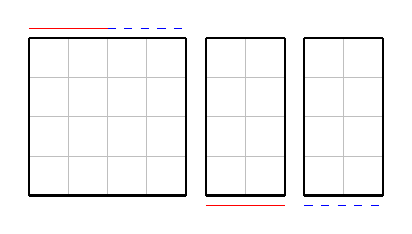
\begin{tikzpicture}[xscale = 1, yscale = 1]
	\draw[lightgray] (0,0) grid [step = 0.5] (2,2);
	%\draw[lightgray] (0,2) grid [step = 0.5] (2,4);
	\draw[thick] (0,0) grid [step = 2] (2,2);
	%\draw[thick] (0,2) grid [xstep = 1, ystep=2] (2,4);
	
	\draw[red] (0,2.125) -- (1,2.125);
	\draw[blue, dashed] (1,2.125) -- (2,2.125);
	
	\begin{scope}[shift={(2.25,0)}]
		\draw[lightgray] (0,0) grid [step = 0.5] (1,2);
		\draw[thick] (0,0) grid [xstep = 1, ystep=2] (1,2);
		\draw[red] (0,-0.125) -- (1,-0.125);
	\end{scope}
	
	\begin{scope}[shift={(3.5,0)}]
		\draw[lightgray] (0,0) grid [step = 0.5] (1,2);
		\draw[thick] (0,0) grid [xstep = 1, ystep=2] (1,2);
		\draw[blue, dashed] (0,-0.125) -- (1,-0.125);
	\end{scope}
	
\end{tikzpicture}
\caption{T-joint. }
\end{subfigure}
\begin{subfigure}{\textwidth}
\centering
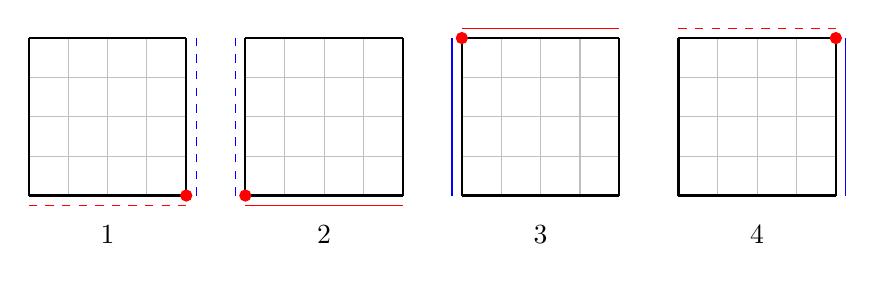
\begin{tikzpicture}[xscale = 1, yscale = 1]
	% grid
	\foreach \x in {0, ..., 3}{
		\begin{scope}[shift={(2.75*\x,0)}]
			\draw[lightgray] (0,0) grid [step = 0.5] (2,2);
			\draw[thick] (0,0) grid [step = 2] (2,2);
			%\draw[fill = red, color=red]  (2,2) circle (2pt);
			%\node at (1,0) {\x};
		\end{scope}
	}
	
	\node at (1,-0.5) {1};
	\node at (1+2.75,-0.5) {2};
	\node at (1+2.75*2,-0.5) {3};
	\node at (1+2.75*3,-0.5) {4};
	
	% Xpoint
	\draw[fill = red, color=red]  (2,0) circle (2pt);
	\draw[fill = red, color=red]  (2.75,0) circle (2pt);
	\draw[fill = red, color=red]  (2.75*2,2) circle (2pt);
	\draw[fill = red, color=red]  (2+2.75*3,2) circle (2pt);
	
	% Interfaces
	\draw[red] (0+2.75,-0.125) -- (2+2.75,-0.125);
	\draw[red] (0+2.75*2,2.125) -- (2+2.75*2,2.125);
	
	\draw[red, dashed] (0,-0.125) -- (2,-0.125);
	\draw[red, dashed] (0+2.75*3,2.125) -- (2+2.75*3,2.125);
	
	\draw[blue] (-0.125+2.75*2,0) -- (-0.125+2.75*2,2);
	\draw[blue] (2.125+2.75*3,0) -- (2.125+2.75*3,2);
	
	\draw[blue, dashed] (2.125,0) -- (2.125,2);
	\draw[blue, dashed] (-0.125+2.75,0) -- (-0.125+2.75,2);
	
	
\end{tikzpicture}
	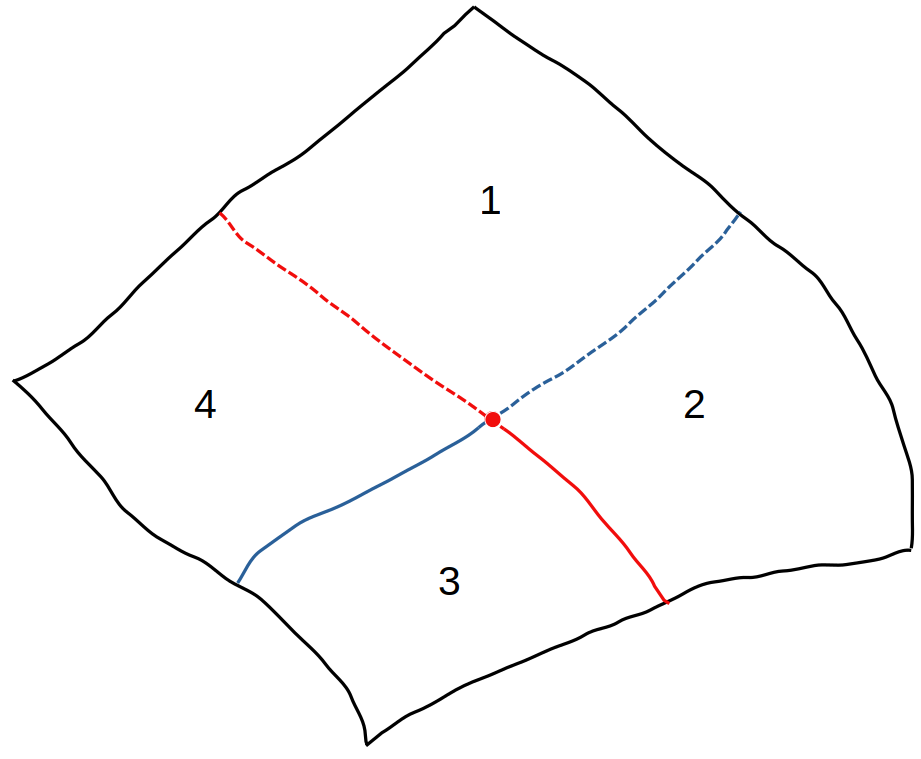
\includegraphics[width=0.4\textwidth]{images/X_point_in_physical.png}
\caption{X-point in logical and physical domain.}
\end{subfigure}
\caption{\label{Patches_logical_dom} Patches in the logical domain.}
\end{figure}

\newpage

\paragraph{}
We want to stay general here and not to focus on one specific decomposition of the domain into patches. The figures Fig. \ref{Complex_geometry_1} and \ref{Complex_geometry_2} give examples of more complex spaces. These are not necessarily for the decomposition of the separatrix.

\begin{figure*}
	\centering
	\includegraphics*[width=0.8\textwidth]{images/5patches_sketch.jpg}
	\caption{\label{Complex_geometry_1}
	          Simple sketch of more complicated geometry with X-point (cyan point). 
			  Physical edges and corners are identified on the logical patches.
			  This illustrates the idea how we intend to represent the multipatch geometry 
			  using tensor-product patches.}
\end{figure*}

\begin{figure*}
	\centering
	\includegraphics*[width=0.8\textwidth]{images/T-joint_sketch.jpg}
	\caption{\label{Complex_geometry_2}
			  Quick sketch of geometry with O-point (purple point) and T-joint (cyan point).
			  There is a T-joint at the cyan point because 
			  edges from patch {\uppercase\expandafter{\romannumeral 2}}
			  and {\uppercase\expandafter{\romannumeral 3}} are connected to the eastern edge
			  of patch {\uppercase\expandafter{\romannumeral 1}}. 
			  Note that the y-dimension of patch {\uppercase\expandafter{\romannumeral 1}}
			  is periodic.}
\end{figure*}

\newpage


\section{Advection equation}
\paragraph{}
We focus on the advection and Poisson equation separately in the context of the questions raised in the introduction. We start with the advection equation. 

\paragraph{}
In the guiding center equations example, the advection equation is given by 
\begin{equation}
\begin{aligned}
	\partial_t \rho + A\cdot\nabla \rho = 0,
\end{aligned}
\label{guiding_center_eq}
\end{equation}

with $A$ the advection field defined on the logical domain on the physical domain axes ($A(r,\theta) = [A_x (r,\theta), A_y(r,\theta)]$). Another example is the advection of the drift-kinetic model 
\begin{equation}
\begin{aligned}
	\partial_t f 
		+ v_{GC}\cdot \nabla_{\perp}f 
		+ v_{\parallel} \partial_z f 
		+ \dot{v}_{\parallel} \partial_{v_{\parallel}} f
		= 0,
\end{aligned}
\end{equation}
but it seems that the multi-patch problems are similar as in the case of the guiding center equations and so we focus on \eqref{guiding_center_eq} only.


\paragraph{Computing the advection field.}
The advection field is computed from the solution of the Poisson equation. In the guiding center equations example,
\begin{equation}
	A = - \nabla \phi \wedge e_z,
\end{equation}

this computation can be done locally. 


\begin{center}
\begin{tabular}{ |l|l| } 
 \hline
 Store 	& $\bullet$ Spline representation (and values?) of $\phi$. \\
 		& $\bullet$ Spline representation (and values?) of $A$. \\
  		& $\bullet$ Jacobian matrix. \\
 \hline
\end{tabular}
\end{center}


\paragraph{Solving the characteristic equation. }
The equation to solve is 
\begin{equation}
\left\{
\begin{aligned}
	& \partial_t X(t; s, x)  = A(t,X(t; s, x)), \\
	& X(s; s, x) = x.
\end{aligned}
\right.
\end{equation}


we compute 
\begin{equation}
\left\{
\begin{aligned}
	& \partial_t X(t^{n}; t^{n+1}, x)  = A(t, X(t^{n}; t^{n+1}, x)), \\
	& \hat{X}(t^{n}; t^{n+1}, x) = \bar{\psi} (t^{n}; t^{n+1}, x)
\end{aligned}
\right.
\end{equation}

where $\bar{\psi}$ is a discrete flow computed with
a time integration method. In the case of Runge-Kutta method, the advection field needs to be evaluated at intermediate feet.

\paragraph{\textit{Example of RK2.}}
\begin{equation}
\begin{aligned}
	& X^1 = X^0 - \frac{dt}{2} A(X^0), \\
	& X^2 = X^0 - dt A(X^1). \\
\end{aligned}
\end{equation}


\paragraph{Outside the patch.}
In case of $X^1$ is outside the patch we are working on, we need to communicate with the other patches to evaluate the advection field. 
The same problem appears when we have solved the characteristic equation and want to evaluate the advected function $\rho$. 


\begin{figure}[!h]
\centering
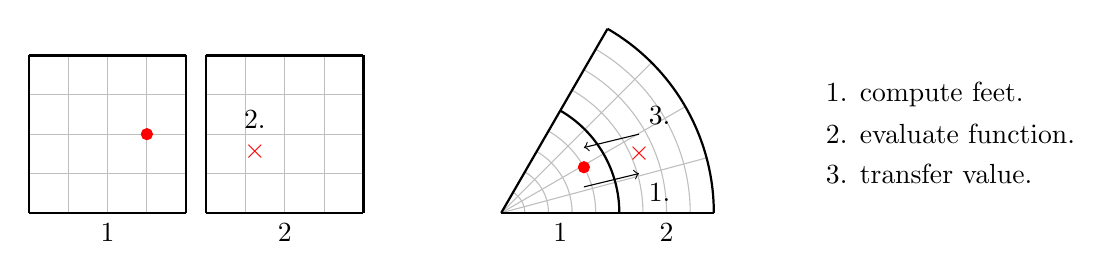
\begin{tikzpicture}[xscale = 1, yscale = 1]
	% logical grid 
	\draw[lightgray] (0,0) grid [step = 0.5] (2,2);
	\draw[thick] (0,0) grid [step = 2] (2,2);
	\node at (1, -0.25) {$1$};
	
	\begin{scope}[xshift=2.25cm]
		\draw[lightgray] (0,0) grid [step = 0.5] (2,2);
		\draw[thick] (0,0) grid [step = 2] (2,2);
		\node at (1, -0.25) {$2$};
	\end{scope}
	
	% feet
	\draw[fill = red, color=red]  (1.5,1) circle (2pt);
	\node at (2.87, 0.78) {\color{red} $\times$};
	
	%\draw[dashed, gray, ->] (1.5, 0.75) -- (2.87, 0.53) node[below]{feet}; 
	%\draw[dashed, gray, <-] (1.5, 1.25) -- (2.87, 1.02) node[above]{value}; 
	
	\node at (2.87, 0.78+0.4) {2.};
	
	
	\begin{scope}[xshift=6cm]
		% physical grid
		\def\RmaxA{1.5}
		\def\RmaxB{2.7}
		\foreach \r in {0, 0.3, ...,\RmaxB} {
		    \draw[lightgray] (0,0) ++(0:\r) arc (0:60:\r);
		}
		\foreach \theta in {0, 15, ..., 60} {
    			\draw[lightgray] (0,0) -- (\theta:\RmaxB);
		}
		\node at (0.75, -0.25) {$1$};
		\node at (2.1, -0.25) {$2$};


		\draw[thick, black] (0,0) ++(0:\RmaxA) arc (0:60:\RmaxA);
		\draw[thick, black] (0,0) ++(0:\RmaxB) arc (0:60:\RmaxB);
		
		\draw[thick, black] (0,0) -- (0:\RmaxB);
		\draw[thick, black] (0,0) -- (60:\RmaxB);
		
		% feet
		\draw[fill = red, color=red]  (1.05,0.58) circle (2pt);
		\node at (1.75, 0.75) {\color{red} $\times$};
		
		\draw[->] (1.05, 0.58-0.25) -- (1.75, 0.75-0.25) node[below right]{1.}; 
		\draw[<-] (1.05, 0.58+0.25) -- (1.75, 0.75+0.25) node[above right]{3.}; 
	\end{scope}
	
	% legend
	\begin{scope}[xshift=10cm]	
		\node[right] at (0,1.5) {1. compute feet.};
		\node[right] at (0,1) {2. evaluate function.};
		\node[right] at (0,0.5) {3. transfer value.};
	\end{scope}
\end{tikzpicture}
\caption{Example of a characteristic foot outside the patch 1 in the logical and physical domains.}
\end{figure}

\begin{center}
\begin{tabular}{ |l|l| } 
 \hline
 Exchange 	&  $\bullet$ The outside feet (in the physical domain?). \\
 			&  $\bullet$ The evaluated value of the advection field. \\
 			&  $\bullet$ The evaluated value of the advected function. \\

 \hline
 Store 	& $\bullet$ Spline representation (and values?) of the advected function $\rho$. \\
 		& $\bullet$ Spline representation (and values?) of the advection field $A$. \\
 \hline
\end{tabular}
\end{center}

\paragraph{Further questions on outside feet.}
Problem: the mapping from the logical to the physical domain is not always easily invertible. 

\begin{itemize}
	\item For an advection in the physical domain, if the feet is outside of the domain, how to get the feet in the logical domain of another patch 
	(inverting the mapping for the other patch might be costly)?
	\item For an advection in the pseudo-Cartesian domain, if the feet is outside of the domain, what are the equivalent coordinate in the physical domain? 
\end{itemize}

Two fundamental possibilities:
\begin{enumerate}
	\item \textbf{Advect in physical domain}: If necessary, use control points of the spline mapping
			to find the patch and then invert the spline mapping to get logical coordinates
			(preferred by Eric),
	\item \textbf{Advect in logical/pseudo-cartesian domain}: Extend the coordinates of the patch
			and find coordinate transformation to logical coordinates of neighboring patches (we do not know yet how to do this, it is just an idea).
\end{enumerate}

If the field lines do not cross the edge (ex. inside of the core), the characteristics do not cross the edge often and 
in these cases inverting a spline mapping might be feasible. Maybe a clever combination of using logical and 
physical coordinates in certain situations is the best approach?


\begin{figure}[!h]
\begin{subfigure}{0.33333\textwidth}
\centering
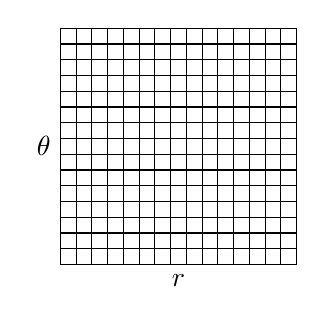
\begin{tikzpicture}[xscale = 2, yscale = 2]
    \draw (0,0) grid[step=0.1] (1.5,1.5);
    %\draw (0.03,0) -- (0.03,1.5);
    %\draw (1.47,0) -- (1.47,1.5);
    \draw (0.75,0) node[below]{$r$};
    \draw (0,0.75) node[left]{$\theta$};
\end{tikzpicture}
\caption{Logical domain.}
\end{subfigure}
\begin{subfigure}{0.33333\textwidth}
\centering
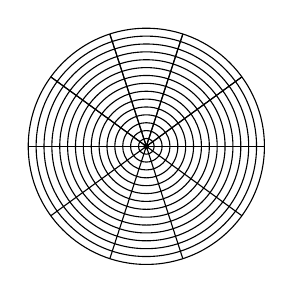
\begin{tikzpicture}[xscale = 1, yscale = 1]
	\foreach \r in {0, 0.1, 0.2, ..., 1.5}
		{\draw (0,0) circle (\r);}
	\draw (0,0) circle (0.03);
%	\draw (0,0) circle (1.47);
	
	\draw (0,0) -- (1.5*1,        1.5*0);
	\draw (0,0) -- (1.5*0.80902,  1.5*0.58779);
	\draw (0,0) -- (1.5*0.30902,  1.5*0.95106);
	\draw (0,0) -- (1.5*-0.30902, 1.5*0.95106);
	\draw (0,0) -- (1.5*-0.80902, 1.5*0.58779);
	\draw (0,0) -- (1.5*-1,       1.5*0);
	\draw (0,0) -- (1.5*-0.80902, 1.5*-0.58779);
	\draw (0,0) -- (1.5*-0.30902, 1.5*-0.95106);
	\draw (0,0) -- (1.5*0.30902,  1.5*-0.95106);
	\draw (0,0) -- (1.5*0.80902,  1.5*-0.58779);
	\draw (0,0) -- (1.5*1,        1.5*0);
	\draw (0,0) -- (1.5*0.80902,  1.5*0.58779);
	\draw (0,0) -- (1.5*0.30902,  1.5*0.95106);
	\draw (0,0) -- (1.5*-0.30902, 1.5*0.95106);
	\draw (0,0) -- (1.5*-0.80902, 1.5*0.58779);
	\draw (0,0) -- (1.5*-1,       1.5*0);

\end{tikzpicture}
\caption{Pseudo-Cartesian domain.}
\end{subfigure}
\begin{subfigure}{0.33333\textwidth}
\centering
	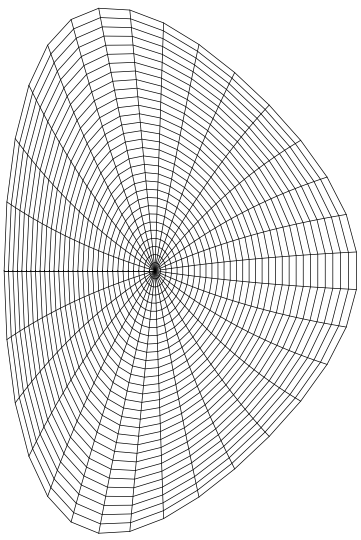
\includegraphics[height=4cm]{images/Czarny_mapping.png}
\caption{Physical domain.}
\end{subfigure}
\end{figure}


\begin{itemize}
	\item How to communicate the feet and values from a patch to another? 
\end{itemize}

Two ideas: 
\begin{enumerate}
	\item Communicate the feet to a global space class; 
		compute in which patch the feet are; 
		evaluate the function at the feet in the right patch; 
		communicate the feet to a global space class to redistribute the values to the first patch.
		
	\item Add some ghost cells around each patch ; update the function values at each every time they change.
\end{enumerate}

\begin{figure}[!h]
\centering
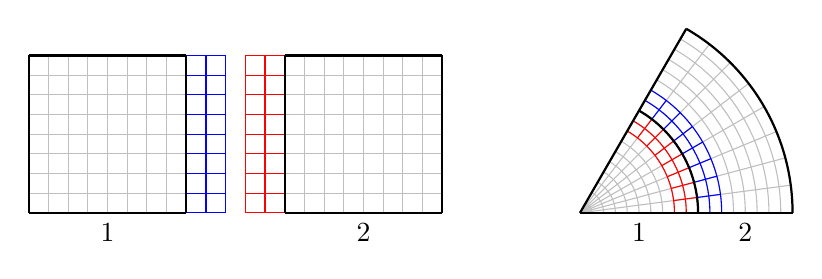
\begin{tikzpicture}[xscale = 1, yscale = 1]
	% logical grid 
	\draw[blue] (2,0) grid [step = 0.25] (2.5,2);
	%\draw[color=white, fill=white] (0,0) -- (0,2) -- (2,2) -- (2,0) -- (0, 0) --cycle;
	\draw[lightgray] (0,0) grid [step = 0.25] (2,2);
	\draw[thick] (0,0) grid [step = 2] (2,2);
	\node at (1, -0.25) {$1$};
	
	\begin{scope}[xshift=3.25cm]
		\draw[red] (-0.5,0) grid [step = 0.25] (0,2);
		\draw[lightgray] (0,0) grid [step = 0.25] (2,2);
		\draw[thick] (0,0) grid [step = 2] (2,2);
		\node at (1, -0.25) {$2$};
	\end{scope}	
	
	\begin{scope}[xshift=7cm]
		% physical grid
		\def\RmaxA{1.5}
		\def\RmaxB{2.7}
		\foreach \r in {0, 0.15, ...,\RmaxB} {
		    \draw[lightgray] (0,0) ++(0:\r) arc (0:60:\r);
		}
		\foreach \theta in {0, 7.5, ..., 60} {
    			\draw[lightgray] (0,0) -- (\theta:\RmaxB);
		}
		\node at (0.75, -0.25) {$1$};
		\node at (2.1, -0.25) {$2$};
		
		% ghost cells
		\foreach \r in {\RmaxA-0.3, \RmaxA-0.15, \RmaxA} {
		    \draw[red] (0,0) ++(0:\r) arc (0:60:\r);
		}
		\foreach \theta in {0, 7.5, ..., 60} {
    			\draw[red] (\theta:\RmaxA-0.3) -- (\theta:\RmaxA);
		}
		
		\foreach \r in {\RmaxA, \RmaxA+0.15, \RmaxA+0.3} {
		    \draw[blue] (0,0) ++(0:\r) arc (0:60:\r);
		}
		\foreach \theta in {0, 7.5, ..., 60} {
    			\draw[blue] (\theta:\RmaxA) -- (\theta:\RmaxA+0.3);
		}


		\draw[thick, black] (0,0) ++(0:\RmaxA) arc (0:60:\RmaxA);
		\draw[thick, black] (0,0) ++(0:\RmaxB) arc (0:60:\RmaxB);
		
		\draw[thick, black] (0,0) -- (0:\RmaxB);
		\draw[thick, black] (0,0) -- (60:\RmaxB);
	\end{scope}
	
\end{tikzpicture}
\caption{Ghost cells for the previous example.}
\end{figure}


For the ghost cells option, we need to know in advance what will be the maximal advection length to not land outside of the ghost cells zone. (Is this length known?) To update the values in the ghost cells, we also need to evaluate the function on the mesh points of the ghost cells of other patches (the mesh points won't always coincide between two patches, especially if we want one more refined than the other). 

For the first option, we need to compute in which patch the feet are (which can be non-trivial).



\paragraph{Build a spline representation of the advected function.}
To do it, we 
\begin{itemize}
	\item Evaluate the spline representation of $\rho$ at the characteristic feet \textbf{[local but need to communicate]}; 
	\item Compute the derivatives at the interfaces of each patch. To do it, there are different methods: 
	\begin{itemize}
		\item advect the derivatives \textbf{[local method]}; 
		\item compute the derivatives by: 
		\begin{itemize}
			\item using Lagrange polynomials \textbf{[neighbor local (only implies 2 patches)]}; 
			\item using global spline relation \textbf{[global method]}. 
		\end{itemize}
	\end{itemize}
	\item Build the new spline representation \textbf{[local]}.
\end{itemize}


\begin{center}
\begin{tabular}{ |l|l| } 
 \hline
 Exchange 	&  $\bullet$ The mesh points around the interfaces for Lagrange interpolation. \\
 			&  $\bullet$ The value of $\rho$ around the interfaces for Lagrange interpolation. \\
 		 	&  $\bullet$ The sum of values of the function $\sum_i \alpha_i s(x_i) = \sum_{p \in patches}\sum_{x_i\in p} \alpha_i s(x_i)$. \\
 \hline
 Store 	& $\bullet$ Spline representation of the advected function $\rho$. \\
 \hline
\end{tabular}
\end{center}




\subsection{Further questions}
\paragraph{About evaluating functions.}
\begin{itemize}
	\item How do we know in which patch we are?
	\begin{itemize}
		\item For a given point in the physical domain, how do we know in which subset it belongs to?
	\end{itemize}
	\item Let's assume we know in which patch we are, how can we evaluate a function? 
			How can we get $\rho(x,y)$ with $(x,y)$ in the physical domain 
			(especially when the mapping difficult to invert)?
	\end{itemize}



% \paragraph{About the space splitting.}
% \begin{itemize}
% 	\item Do we have the splitting of the space from another code?
% 	\item Do we have mappings?
% 	\item If we are using different mappings between the patches, how to stick correctly the patches at the edge? Are not risks of ill-covering (gaps or covering of two patches)? 
% \end{itemize}


\begin{figure}[!h]
\centering
	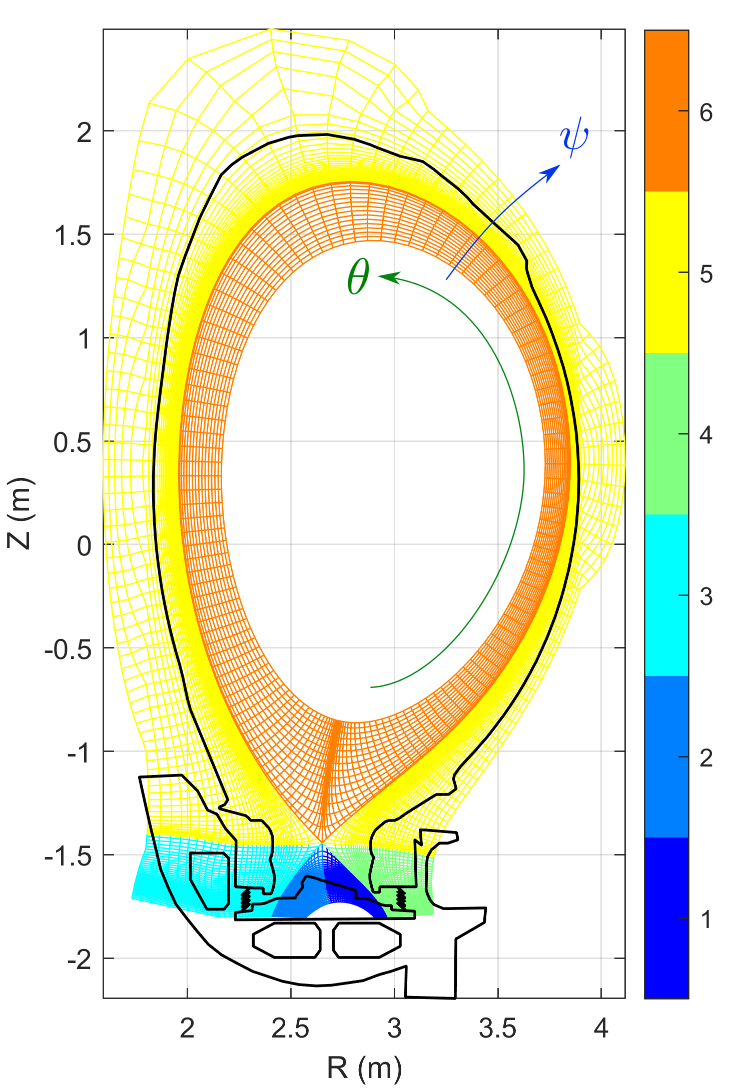
\includegraphics[height=15cm]{images/JET_zones2_SOLEDGE.png}
\caption{Multi-patch decomposition from SOLEDGE.}
\end{figure}

\newpage


\end{document}


